\chapter{Experiments} \label{chp:experiments}

\section{Experimental Setup}
All experiments were conducted on a consistent hardware and software platform to ensure fair and reproducible comparisons. This section details the environment and datasets used in our evaluation.

\subsection{Hardware and Software}
The experimental platform is a MacBook Pro equipped with an Apple M4 Pro processor and 24 GB of RAM, running macOS. Our proposed algorithm was implemented in C++ and it is available at \url{}. We compiled it using Apple Clang 17. 

In particular, we utilized the PathSort algorithm implementation of the XBWT proposed in \cref{sec:xbwt_impl}. Moreover, we used a C++ implementation by Vladimir Kolmogorov of the minimum cost perfect matching algorithm described in \cite{kolmogorovBlossomNewImplementation2009}. The implementation is available at \url{https://pub.ista.ac.at/~vnk/software.html}.

\begin{comment}
In brief, paper \cite{kolmogorovBlossomNewImplementation2009} presents Blossom~V, a practical implementation of Edmonds’ blossom algorithm for computing minimum-cost perfect matchings in undirected weighted graphs. While the theoretical worst-case bounds for the blossom family have steadily improved since Edmonds’ original $O(n^2m)$ algorithm, Blossom~V is designed for strong empirical performance rather than new asymptotic guarantees. It combines two ingredients that had proven effective separately in prior work: the variable $\delta$ (variable dual updates) strategy popularized by Blossom~IV, and systematic use of priority queues to efficiently select minimum-slack edges.

Blossom~V targets general (not necessarily bipartite) graphs, and thus directly applies to our bipartite instances as a special case. In our experiments we use the publicly available Blossom~V implementation as a black-box solver to compute minimum-cost perfect matchings for the graphs generated by our compression pipeline.
\end{comment}

\subsection{Datasets}
To systematically evaluate performance under controlled conditions, particularly with respect to repetitiveness, we generated a suite of synthetic labeled tries. Real-world datasets often lack ground-truth information about their repetitive structures, making it difficult to isolate the effects of this property. Our synthetic generation approach allows us to create trees with tunable characteristics.

The tries were generated using a custom Python script that constructs a tree and introduces repetitiveness by randomly copying subtries to different locations. At each step of the tree's growth, with a certain probability, a random existing subtrie is selected and duplicated as a new branch. This "copy-paste" mechanism allows us to create complex, highly repetitive structures that mimic patterns found in real-world data.

The generation process was controlled by the following key parameters:
\begin{description}
    \item[Max Branching Factor] The maximum number of children for any node.
    \item[Repetition Probability] The probability of copying an existing subtrie instead of creating a new random branch.
    \item[Subtrie Depth Range] The minimum and maximum depth of subtries eligible for copying.
    \item[Max Nodes] The target maximum number of nodes in the generated trie.
    \item[Alphabet Size] The number of unique characters in the alphabet.
    \item[Seed] The seed used for random number generation to ensure reproducibility.
\end{description}

By varying these parameters, we can produce a diverse range of tries to thoroughly test the limits and behaviors of each compression algorithm.

\section{Compression as a Parameter of \texorpdfstring{$p$}{p}}
Our first experiment investigates the relationship between the co-lexicographical width, $p$, of the automaton produced by our compression pipeline and the final compression size. The central hypothesis is that a larger value of $p$ directly leads to a better compression ratio as shown in \cite{manziniRationalConstructionWheeler2024} (see \cref{thm:exp_increase}). 

To generate automata with varying co-lex widths, we controlled the structural repetitiveness of the input tries using the \texttt{repetition\_probability} parameter in our data generator. We conducted two main experiments:

\begin{enumerate}
    \item \textbf{Low-Repetitivity Scenario:} We generated a set of $100$ tries with a target size of 100,000 nodes, an alphabet size of $26$ characters and a low repetition probability of $0.2$.
    \item \textbf{High-Repetitivity Scenario:} We generated a second set of $100$ tries with a target size of 100,000 nodes, an alphabet size of $26$ characters, but with a high repetition probability of $0.8$.
\end{enumerate}

We run our full compression pipeline on each trie with different values of $p$ in range $[1, 15]$. We then report the maximum, mean, and minimum number of nodes and edges obtained after compression. By correlating the measured $p$ with the final compression ratio in both scenarios, we aim to empirically demonstrate that the compression of our method is fundamentally governed by the co-lex width of the resulting automaton.

For each value of $p$, the experimental results are presented as boxplots, which provide a comprehensive statistical summary of the compression performance across all $100$ trials. Each boxplot displays:
\begin{itemize}
    \item The \textbf{median} (middle line): the central value that separates the upper and lower halves of the results.
    \item The \textbf{first quartile (Q1)} and \textbf{third quartile (Q3)} (box boundaries): representing the 25th and 75th percentiles, respectively, with the box containing the middle 50\% of the data.
    \item The \textbf{interquartile range (IQR)}: the spread of the middle 50\% of observations, calculated as Q3 - Q1.
    \item The \textbf{whiskers}: extending to the most extreme data points within 1.5 × IQR from the box boundaries.
    \item \textbf{Outliers}: individual points beyond the whiskers, representing unusually high or low compression ratios.
\end{itemize}
This visualization allows us to assess not only the central tendency of compression performance for each $p$ value, but also the variability and distribution shape of the results across different trie structures. Additionally, the mean compression value for each $p$ is highlighted with a red line plot that is overlaid on the boxplots to show the overall trend.

The results from our experiments, presented in \cref{fig:exp_low_rep} and \cref{fig:exp_high_rep}, confirm that increasing the parameter $p$ leads to a substantial improvement in compression for both low- and high-repetition datasets. As $p$ grows, the number of nodes and transitions in the compressed automaton decreases significantly, demonstrating the effectiveness of the string partitioning approach in identifying and merging MN-equivalent nodes while keeping the co-lexicographical width of the automaton controlled.

\begin{figure}[H]
    \centering
    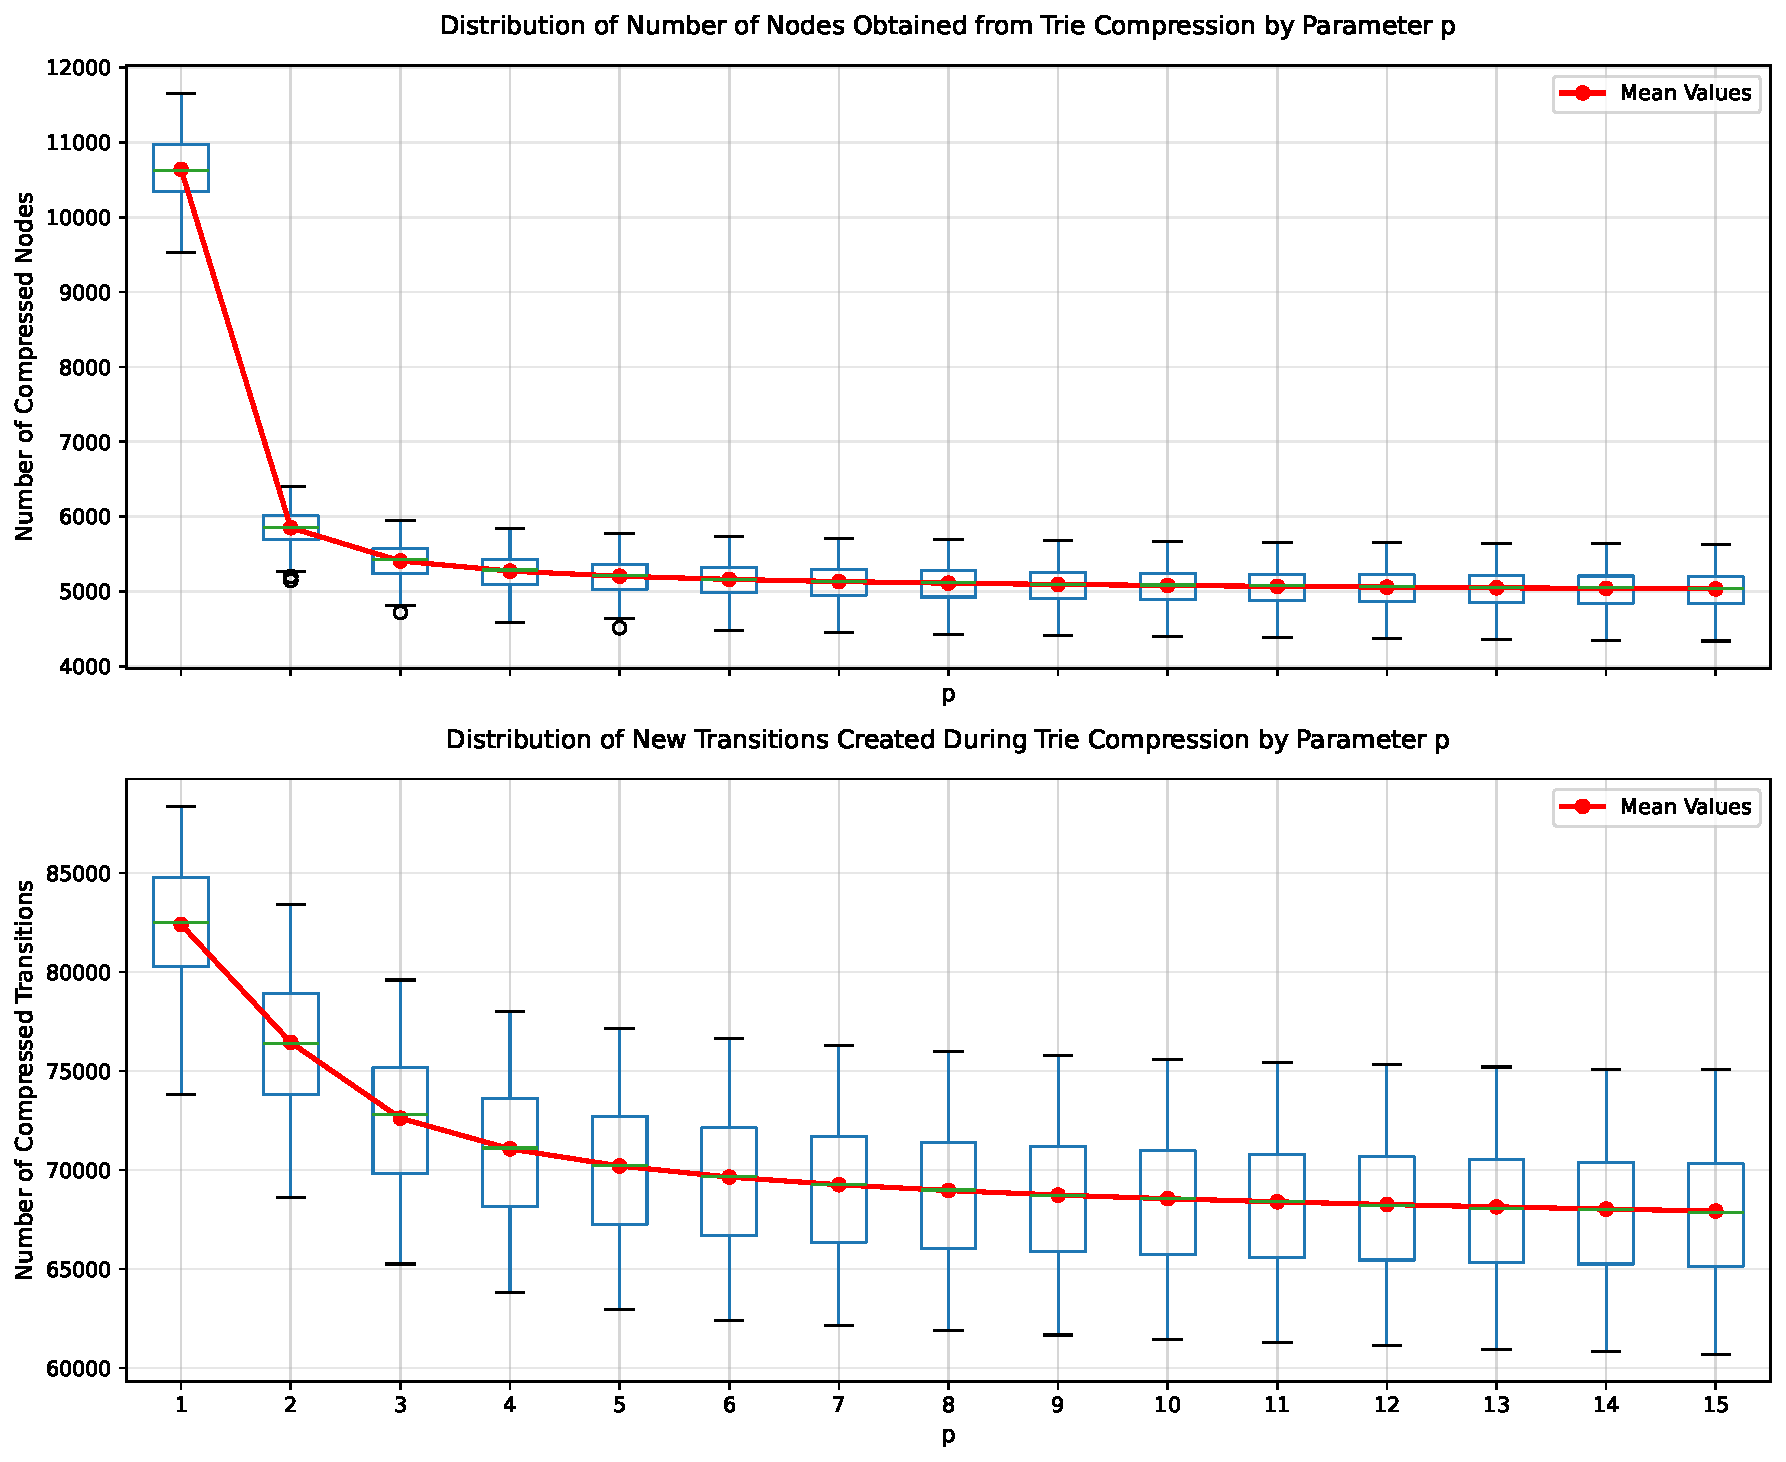
\includegraphics[width=1\linewidth]{Immagini/tree_compression_analysis_low.pdf}
    \caption{Experimental results for the low-repetition scenario. The top plot shows the number of nodes in the compressed trie as a function of $p$, while the bottom plot shows the number of transitions.}
    \label{fig:exp_low_rep}
\end{figure}

\begin{figure}[H]
    \centering
    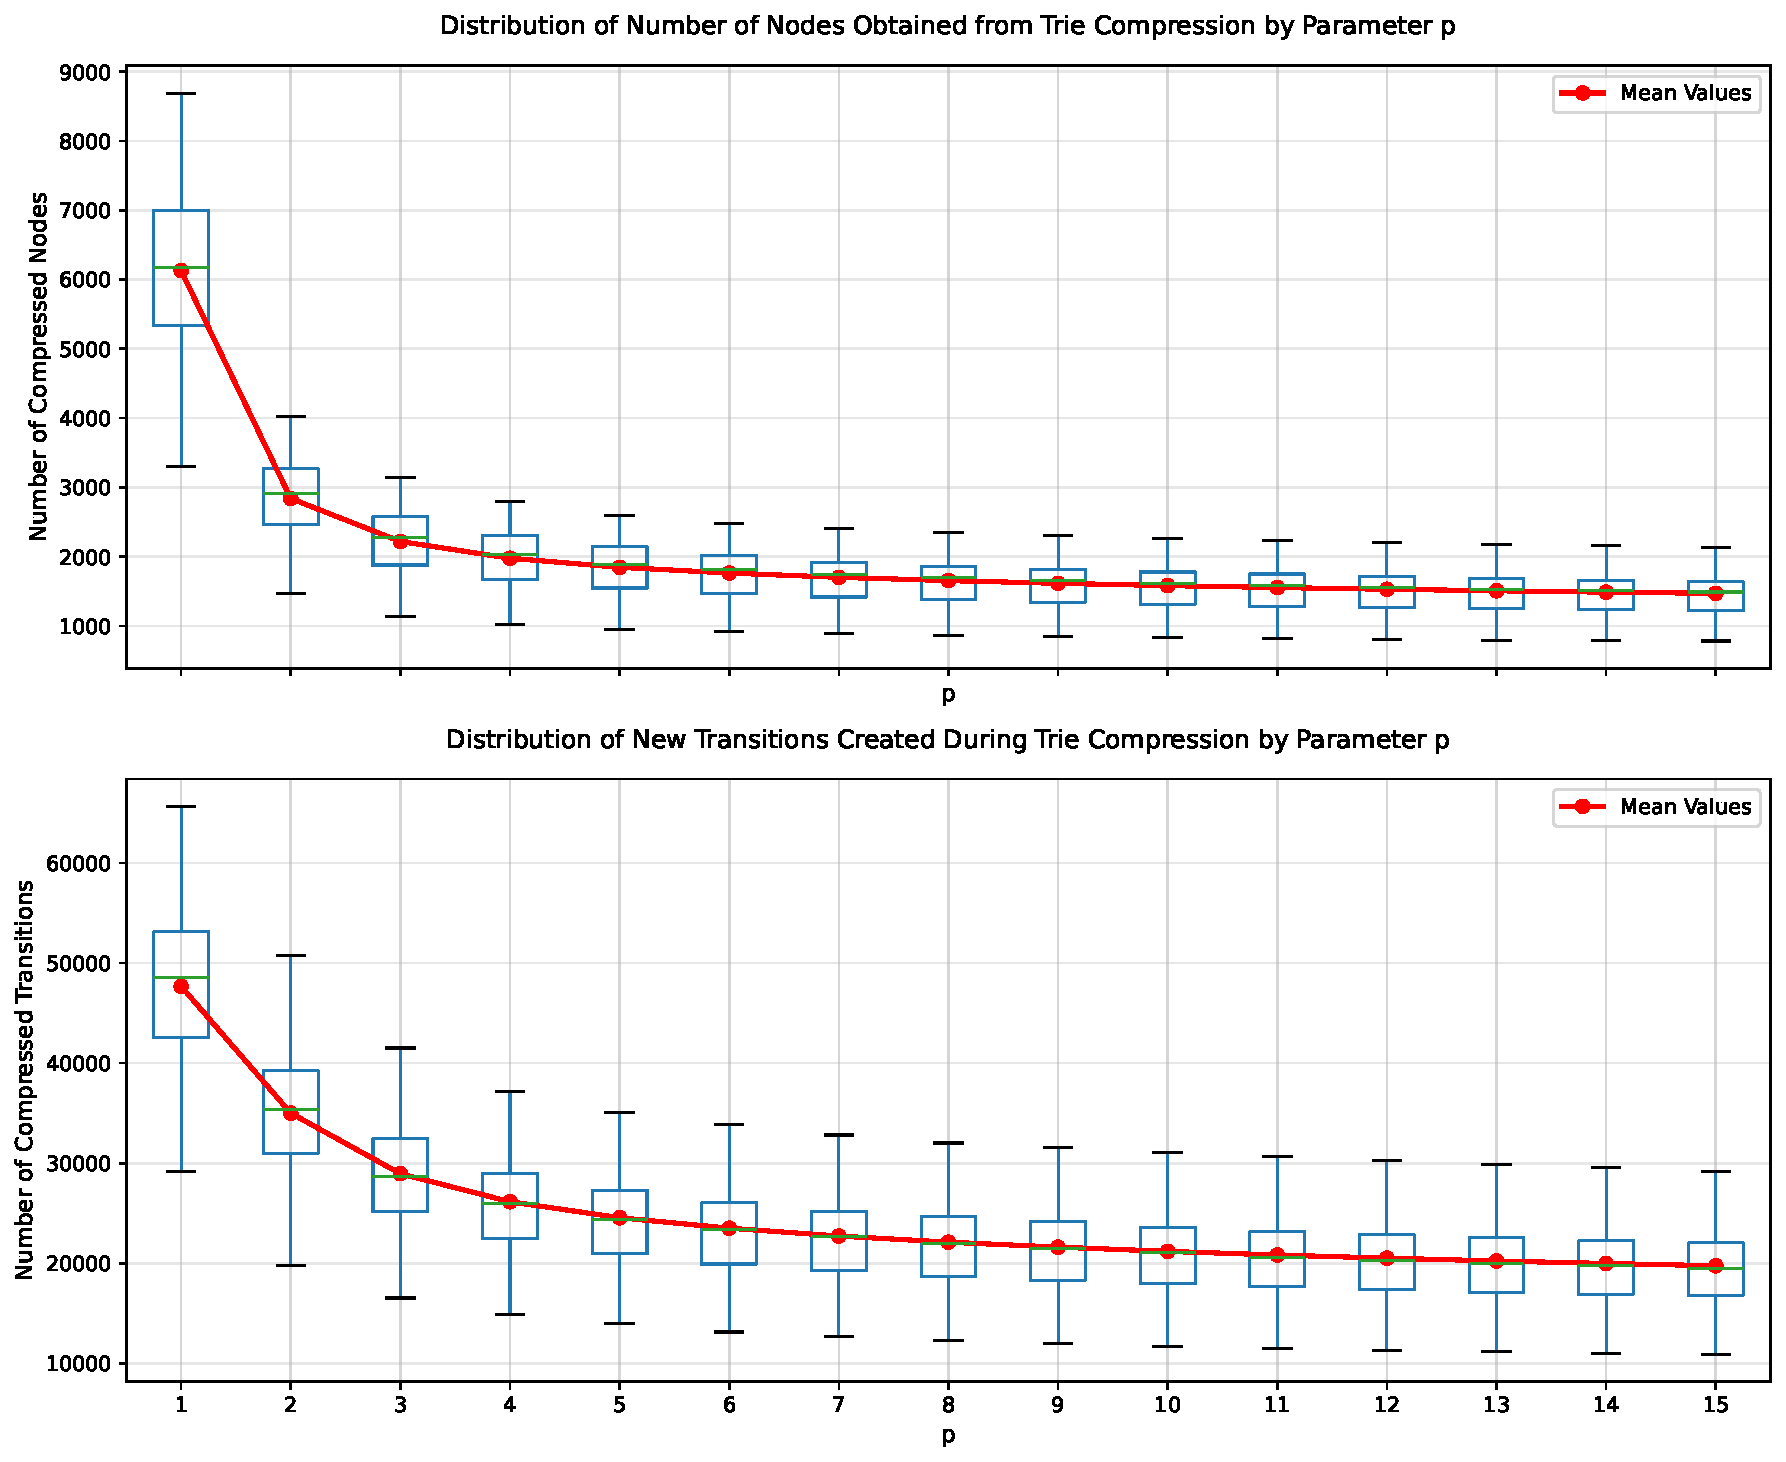
\includegraphics[width=1\linewidth]{Immagini/tree_compression_analysis_high.pdf}
    \caption{Experimental results for the high-repetition scenario. The top plot shows the number of nodes in the compressed trie as a function of $p$, while the bottom plot shows the number of transitions.}
    \label{fig:exp_high_rep}
\end{figure}

To provide a clear comparison between the two scenarios, \cref{fig:exp_comparison} shows the mean and standard deviation for both the low- and high-repetition datasets. The results confirm our hypothesis: tries with higher string repetitiveness achieve significantly better compression, as evidenced by the lower number of nodes and transitions for all values of $p$. This is expected, as a more repetitive trie allow for a more compact representation in the compressed automaton.

\begin{figure}[H]
    \centering
    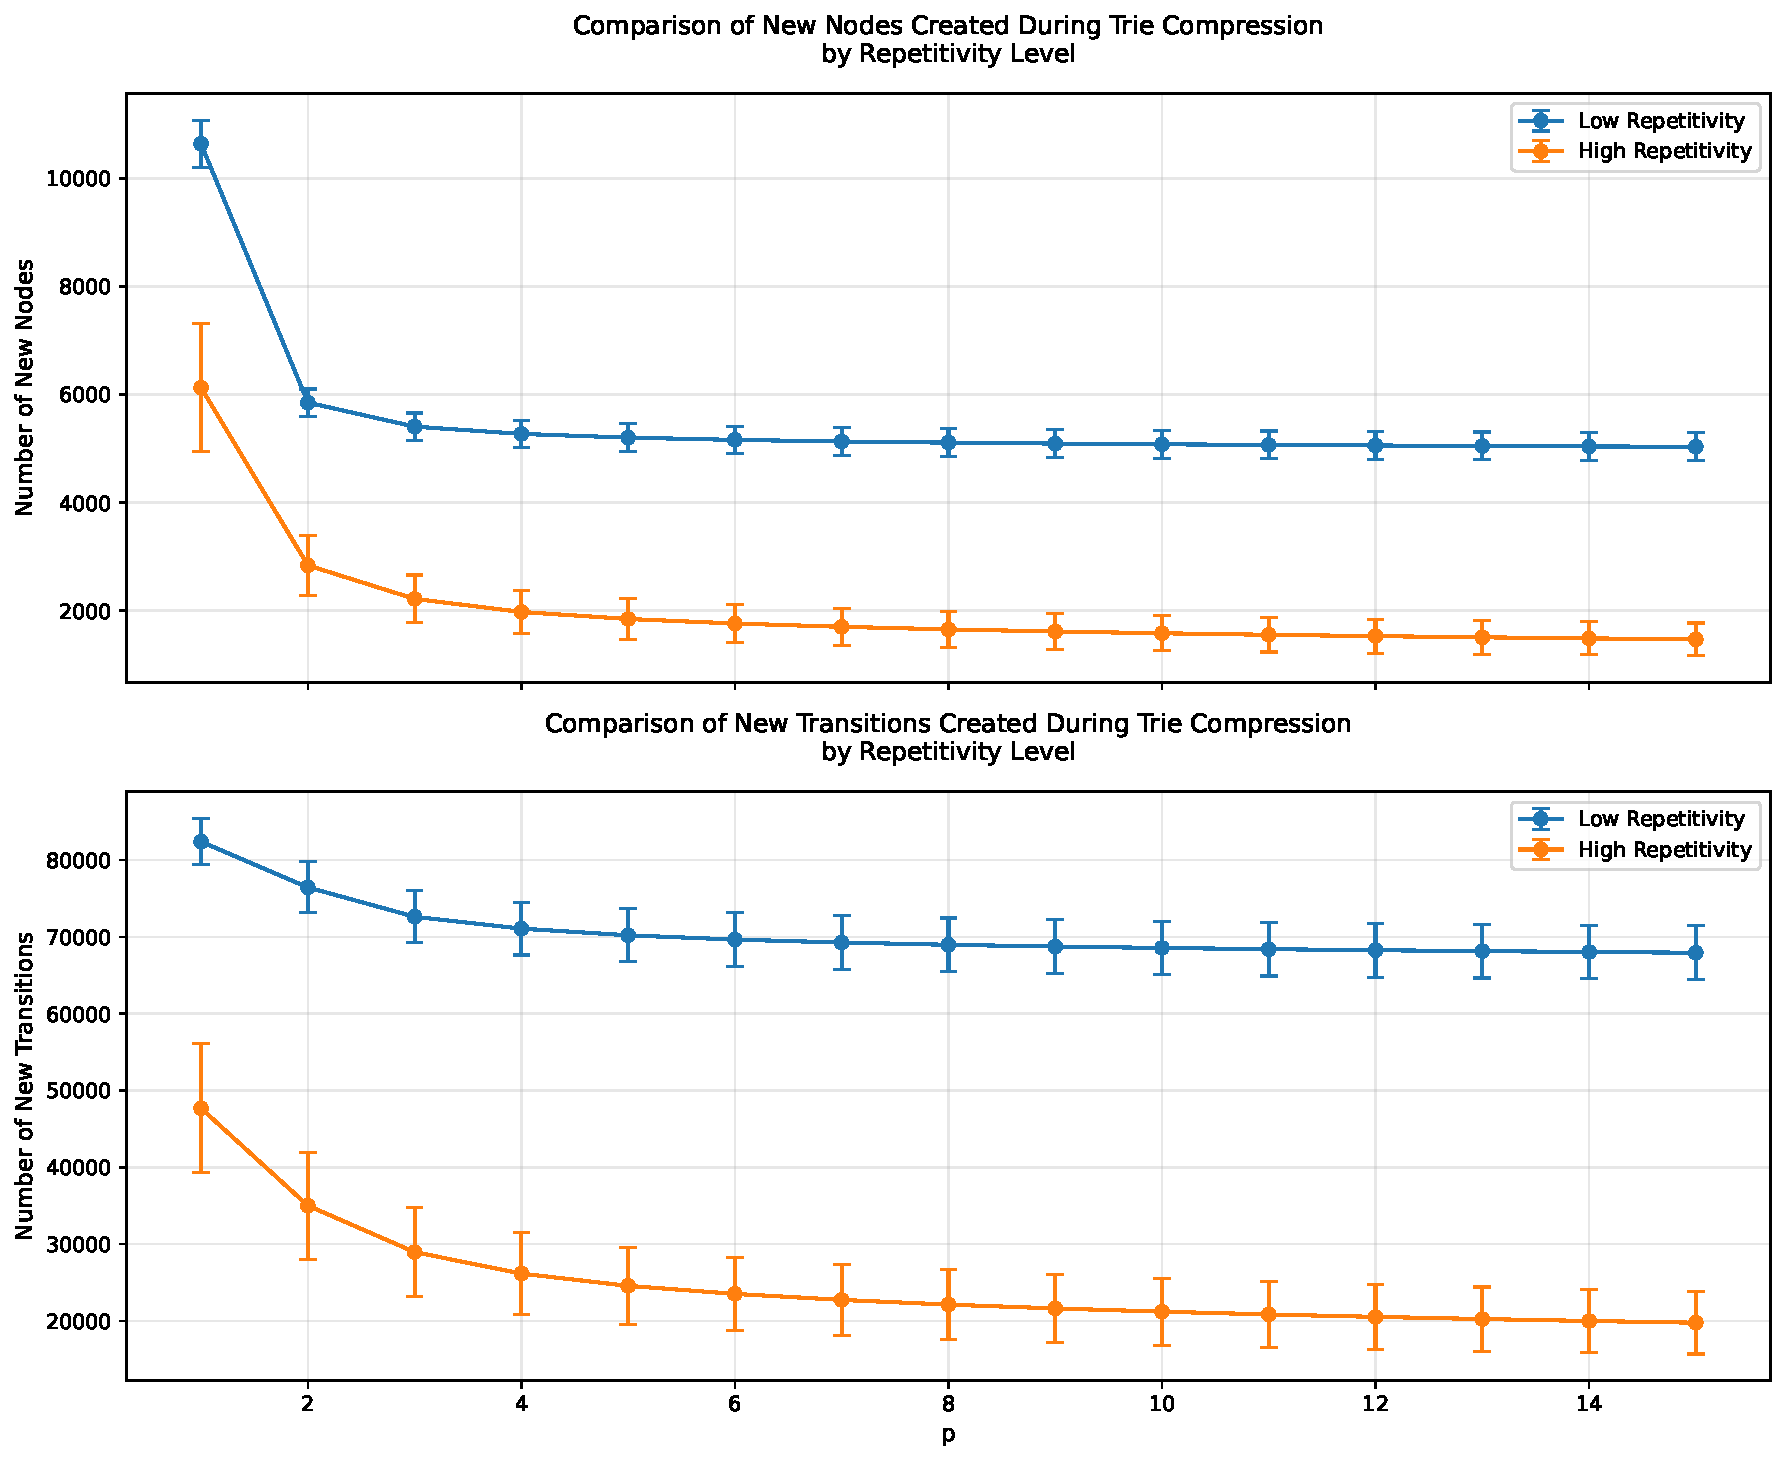
\includegraphics[width=1\linewidth]{Immagini/high_low_comparison.pdf}
    \caption{Comparison of compression performance between the low-repetition and high-repetition scenarios. The top plot compares the number of nodes, and the bottom plot compares the number of transitions.}
    \label{fig:exp_comparison}
\end{figure}